\section{Efficient Enumeration of Laddder Lotteries and its Application}

%%Intro
\subsection{Introduction}
In their paper, \textbf{Efficient Enumeration of Ladder Lotteries and its Application},
the authors provide an algorithm for generating $OptL\{\pi\}$ 
for any $\pi$, in $\mathcal{O}(1)$ per ladder \cite{A1}. This is the first algorithm for generating $OptL\{\pi\}$. 
To see this algorithm please refer to 
Alg.\ref{Alg:FindAllChildren}. The paper also presents the number 
of ladder lotteries in $OptL\{(11, 10, 9, 8, 7, 6, 5, 4, 3, 2, 1)\}$ which is 
$5,449,192,389,984$ \cite{A1}.There are also four other algorithms in 
this section, none of which are found in the paper \emph{Efficient Enumeration of Ladder Lotteries and its Applications}. The 
algorithms are Alg.\ref{Alg:RootLadder}, Alg.\ref{Alg:RightSwap}, Alg.\ref{Alg:LeftSwap} and Alg.\ref{Alg:ShiftChildren}.
These algorithms are used to perform mandatory steps in \ref{Alg:FindAllChildren}. These algorithms are novel.\par 
The authors' algorithm is known as \emph{FindAllChildren}. It is based on several key concepts, the most 
important of which is the \emph{local swap operation}. This is the 
minimal change operation that transitions from one ladder in $OptL\{\pi\}$ to the 
next ladder. The local swap operation is essentially a 180 degree rotation
of three bars in the ladder, such that the bottom
bar is rotated to the top, the middle bar stays in the middle and the top bar
is rotated to the bottom. If the bars undergo a 180 degree rotation to the right, 
then this is known as a \emph{right swap operation} and 
if the bars udergo a 180 degree rotation to the left then this 
is known as a \emph{left swap operation} \cite{A1}. To go to the next ladder in the set, 
the current ladder, $l_{i}$, udergoes a right swap operation 
to get to ladder $l_{i+1}$. See Fig.\ref{fig:rightSwap} for an exmaple of a 
local swap operation. The \emph{route} of an element is the sequence of bars in the ladder that an element must cross 
in order to reach its correct position in 
the identity permutation \cite{A1}. The sequence is ordered from top left to bottom right.
Note, that each bar has two elements that cross it, 
therefore the bar belongs to the route of the greater of the two elements. 
It is important to note that when a right swap operation occurs, 
two of the three bars belong to the route of a unique greater element and one bar belongs
to the route of a unique lesser element. Once rotated, the bar of the lesser element is 
moved above the bars of the greater element.\par
The \emph{clean level} refers to the smallest element 
in $\pi$ such that none of its bars have undergone a right swap operation \cite{A1}.
If there is no such element, then the clean level is the maximum element in $\pi$ + 1.
The \emph{root ladder} is the only ladder in  the set with a clean level of 1; in 
other words, the root ladder is the only ladder in which no bars have undergone 
a right swap operation. The root ladder is unique to $OptL\{\pi\}$. To see the root ladder 
of $OptL\{(4,5,6,3,1,2)\}$ please refer to figure Fig.\ref{fig:root}. The root ladder is
also the \emph{first ancestor  ladder} in $OptL\{\pi\}$. Insofar as the enumeration algorithm 
is based on performing a right swap operation on a pervious ladder, then every other 
ladder in $OptL\{\pi\}$ must have at least one right swap operation. Since the root ladder has
no right swap operations, then it must be an ancestor of every other ladder.\par

%%Root ladder subsection
\subsection{The Root Ladder in Detail}
The authors provide a good description of the root ladder, however they do not provide an algorithm 
for creating the root ladder. Since the root ladder is an ancestor to every other ladder in $OptL\{\pi\}$, 
the root ladder cannot be created using the same algorithm as every other ladder. This thesis provides such 
an algorithm in Alg.\ref{Alg:RootLadder}.\par

\begin{algorithm}
	%%\setstretch{1.35}
	 %% \algsetup{linenosize=\tiny}
	\begin{algorithmic}[1]
		\Function {CreateRoot}{$ladder[2(N-1)-1][N-1]$, $\pi$, $N$, $row \gets 1$}
			\If{$N=1$}
				\State return
			\EndIf
			\State $largestIndex \gets$ index of largest element in $\pi$
			\For{$i \gets largestIndex+1$, $i \leq N$, $i \gets i+1$}
				\If{$\pi_{largestIndex}>\pi_{i}$ $AND$ $largestIndex < i$}
					\State $column \gets i$
					\If{This is the first bar to be added}
						\While{bar cannot be added}
							\State $row \gets row+1$
						\EndWhile
						\State $ladder[row][column] \gets 1$
					\Else 
						\State $row \gets row+1$
						\State $ladder[row][column] \gets 1$
					\EndIf
				\EndIf
			\EndFor
			\State $\pi \gets \pi - largestElement$
			\State $CreateRoot(ladder, \pi, N-1, row \gets 1)$
		\EndFunction

	\end{algorithmic}
	\caption{The algorithm for creating the root ladder of $OptL\{\pi\}$}
	\label{Alg:RootLadder}
\end{algorithm}\pagebreak



Let $ladder$ be a two dimensional array, let $\pi$ be the current state of the permutation, let $N$ be the 
size of $\pi$, let $row$ be the current row in the ladder. First, the index of the largest element in $\pi$ is assigned to $largestIndex$. 
Once found, the algorithm loops from $largestIndex+1$ to $N$. If $\pi_{largestIndex}>\pi_{i}$ then a bar is to be added to 
$ladder$ at $row,column=i$. There are two cases for calculating the $row$. 
\case{\emph{First bar is being added}}{This is the first bar to be added to the route of the largest element. 
$row$ is incremented until a bar can be added to $ladder$ at $row$ 
and $column$. A bar can be added if neither of its endpoints are touching the endpoints of any other bar.}
\case{\emph{Second or greater bar is being added}}{If this is second or greater bar to be added to the route of the 
largest element in $\pi$ then $row \gets row+1$.}
Once all the bars for the route of the largest element have been added, the largest element from $\pi$ is removed, 
$N \gets N-1$ and $row \gets 1$. Then the algorithm makes a recursive call.

\begin{lemma}
	The time complexity for $CreateRoot$ is $O(N^{3})$
\end{lemma}
\begin{proof}
	The outer for-loop of the function runs from some arbitrary index to $N$ on each function call. The inner for loop runs at most 
	$2(N-1)-1$ times which is reduced to $N$. Thus, we get $O(N^{2})$. The following 
	recursion holds, $CreateRoot(N-K) = CreateRoot(N-K+1) + O((N-K)^{2})=CreateRoot(N-K+2) + O((N-K)^{2}) + O((N-K+1)^{2})\dots $. Which is 
	reduced to $O(N(N+1)(2N+1)/6) = O(N^3)$. QED.
\end{proof}
\pagebreak


\begin{figure}[!htp]
	\begin{minipage}{0.4\textwidth}
		\begin{center}

			%%drawing the lines
			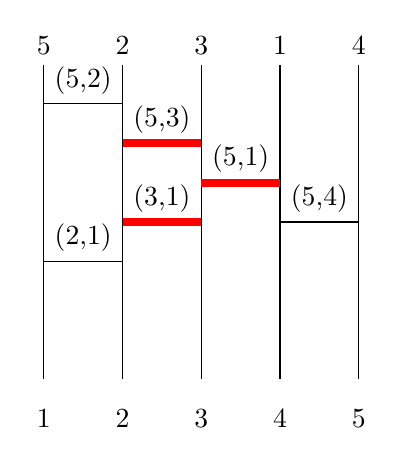
\begin{tikzpicture}
				\draw(0, 0) to (0, 4) node[above]{5};
				\node at (0, -0.5){1};

				\draw(1, 0) to (1, 4) node[above]{2};
				\node at (1, -0.5){2};


				\draw(2, 0) to (2, 4) node[above]{3};
				\node at (2, -0.5){3};

				\draw(3, 0) to (3, 4) node[above]{1};
				\node at (3, -0.5){4};


				\draw(4, 0) to (4, 4) node[above]{4};
				\node at (4, -0.5){5};

				%%drawing the bars

				%%5's route
				\draw(0, 3.5)to (1, 3.5);
					\draw node at (0.5, 3.8) {(5,2)};
				\draw[line width=1mm, red](1, 3) to (2, 3);
					\draw node at (1.5, 3.3) {(5,3)};
				\draw[line width=1mm, red](2, 2.5) to (3, 2.5);
					\draw node at (2.5, 2.8) {(5,1)};
				\draw(3, 2) to (4, 2);
					\draw node at (3.5, 2.3) {(5,4)};

				%%4's route, no bars

				%%3s route
				\draw[line width=1mm, red](1, 2) to (2, 2);
					\draw node at (1.5, 2.3) {(3,1)};
				%%2s route
				\draw(0, 1.5) to (1, 1.5);
					\draw node at (0.5, 1.8){(2,1)};
			\end{tikzpicture}
		\end{center}
	\end{minipage}
	\begin{minipage}{0.4\textwidth}
		\begin{flushright}

			%%drawing the lines
			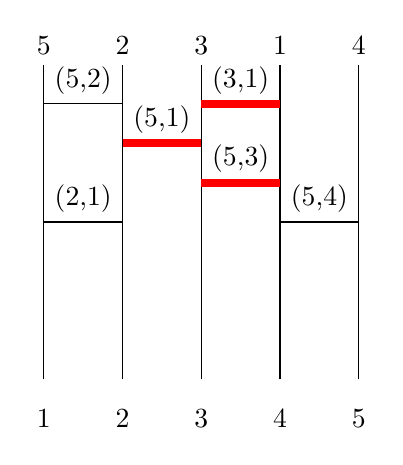
\begin{tikzpicture}
				\draw(0, 0) to (0, 4) node[above]{5};
				\node at (0, -0.5){1};

				\draw(1, 0) to (1, 4) node[above]{2};
				\node at (1, -0.5){2};


				\draw(2, 0) to (2, 4) node[above]{3};
				\node at (2, -0.5){3};

				\draw(3, 0) to (3, 4) node[above]{1};
				\node at (3, -0.5){4};


				\draw(4, 0) to (4, 4) node[above]{4};
				\node at (4, -0.5){5};

				%%Drawing the bars
				\draw(0, 3.5)to (1, 3.5);
					\draw node at (0.5, 3.8){(5,2)};
				\draw[line width=1mm, red](2, 3.5) to (3, 3.5);
					\draw node at (2.5, 3.8) {(3,1)};
				\draw[line width=1mm, red](2, 2.5) to (3, 2.5);
					\draw node at (2.5, 2.8) {(5,3)};
				\draw(3, 2) to (4, 2);
					\draw node at (3.5, 2.3){(5,4)};
				%%4's route, no bars

				%%3s route
				\draw[line width=1mm, red](1, 3) to (2, 3);
					\draw node at (1.5, 3.3) {(5,1)};
				%%2s route
				\draw(0, 2) to (1, 2);
					\draw node at(0.5, 2.3){(2,1)};
			\end{tikzpicture}
		\end{flushright}
	\end{minipage}
	\caption{Example of a local swap operation. When a right swap operation is permformed
	on the left ladder, the result is the right ladder. When a left swap operation is permformed
	on the right ladder, the result is the left ladder.}
	\label{fig:rightSwap}
\end{figure}


\begin{figure}


	\begin{center}
		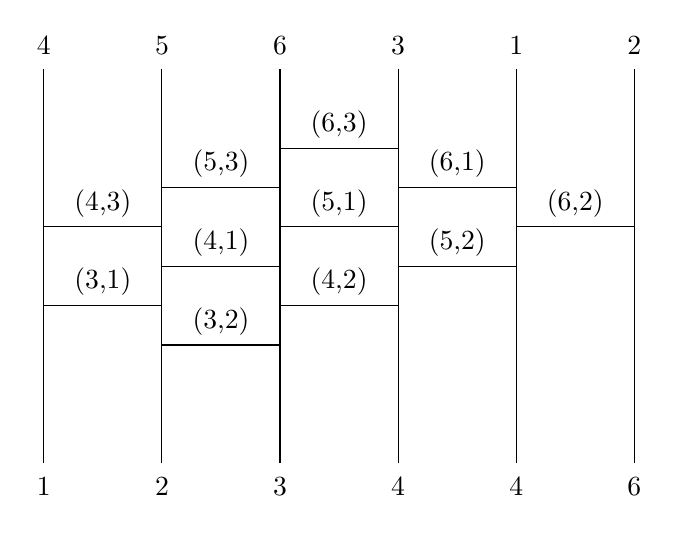
\begin{tikzpicture}
			%%draw the lines
			\draw(0, 0) to (0, 5);
				\node at (0, 5.3){4};
				\node at (0, -0.3){1};

			\draw(1.5, 0) to (1.5, 5);
				\node at (1.5, 5.3){5};
				\node at (1.5, -0.3){2};
			
			\draw(3, 0) to (3, 5);
				\node at (3, 5.3){6};
				\node at (3, -0.3){3};
			\draw(4.5, 0) to (4.5, 5);
				\node at (4.5, 5.3){3};
				\node at (4.5, -0.3){4};
			\draw(6, 0) to (6, 5);
				\node at (6, 5.3){1};
				\node at (6, -0.3){4};
			\draw(7.5, 0) to (7.5, 5);
				\node at (7.5, 5.3){2};
				\node at (7.5, -0.3){6};

			%%draw the bars
			
			%%6's route
			\draw(3, 4) to (4.5, 4);
				\node at (3.75, 4.3){(6,3)};
			\draw(4.5, 3.5) to (6, 3.5);
				\node at (5.25, 3.8){(6,1)};
			\draw(6, 3) to (7.5, 3);
				\node at (6.75, 3.3){(6,2)};
			%%5's route
			\draw(1.5, 3.5) to (3, 3.5);
				\node at (2.25, 3.8){(5,3)};
			\draw(3, 3) to (4.5, 3);
				\node at (3.75, 3.3){(5,1)};
			\draw(4.5, 2.5) to (6, 2.5);
				\node at (5.25, 2.8){(5,2)};
			%draw 4's route
			\draw(0, 3) to (1.5, 3);
				\node at (0.75, 3.3){(4,3)};
			\draw(1.5, 2.5) to (3, 2.5);
				\node at (2.25, 2.8){(4,1)};
			\draw(3, 2) to (4.5, 2);
				\node at (3.75,2.3){(4,2)};

			%%draw 3's route
			\draw(0, 2) to (1.5, 2);
				\node at (0.75, 2.3){(3,1)};
			\draw(1.5, 1.5) to (3, 1.5);
				\node at (2.25, 1.8){(3,2)};
		\end{tikzpicture}

	\end{center}





	\caption{The root ladder for $OptL\{(4,5,6,3,1,2)\}$. Notice how 
	none of the bars have undergone a right swap operation. This is clear 
	when considering that there is no bar of a lesser element above the bar(s)
	of a greater element.} 
	\label{fig:root}

\end{figure}

 %%Save this section for the counting section.
 \begin{theorem}
	 If a ladder from $OptL\{\pi\}$ has not undergone any right swap operations then the ladder is the root ladder. 
	 \label{Theorem:One}
 \end{theorem} 
 \begin{proof}
     The root ladder is defined as the ladder whose clean level is one.
     This means there is no bar of a lesser element above the route a 
     greater element. Keeping in mind that the clean level of the root ladder is one, next consider what is meant by a \emph{child bar}
      which is a bar to the bottom left or right of an arbitrary bar $x$. Within the context of the root ladder, 
      if the left endpoint of the child bar is directly below the right end point of $x$ then the child is a 
     \emph{right child} of $x$. If the right end point of the child bar is directly 
     below the left end point of $x$ then it is a \emph{left child}. Let $x$ belong to the route of element $m$/$Route(m)$.
     If a child is a right child of $x$
	 then it also belongs to the $Route(m)$.
     Let $x$ be a bar representing an inversion with element $m$ and $k$.
     The right child of $x$ is a bar which represents an inversion 
     with $m$ and some element to the right of $k$ termed $k'$. Suppose this was not the case, 
     then this would mean that the right child of $x$ was either a bar representing an inversion 
	 between some element $m'$ such that $m' > m$ or $m' < m$. If $m' > m$ 
	 then this would be a contradiction seeing as $x$ would be above the bar of a route 
     of a greater element which contradicts the definition of the root ladder. On the other hand if 
	 $m' < m$ then $m$ would form an inversion with $m'$ and $x$ would be the bar that uninverted $m$ and $m'$, 
	 but this is also a contradiction seeing as $m' \neq k$ but $x$ uninverts $m$ and $k$. Thus, the right child 
     of $x$ belongs to the same route as $m$ in the root ladder.\par The left child of $x$
     belongs to $Route(l=m-1)$. Suppose this was not the case, 
     then the left child could belong to a route $\geq m$, but if that were the case, this contradicts 
	 the definition of the root ladder seeing as $x$ would be above the route of a greater element. If 
	 $l < m-1$ then the left child of $x$ would be above $Route(m-1)$ which also contradicts the definition 
	 of the root ladder. Therefore, the left child of $x$ must belong to route $l=m-1$. 
	 The second element of the left child of $x$ is $k$. Suppose this was not the case, then 
	 let the second element of the left child be termed $k'$. 
	 $k'$ forms an inversion with $m-1$. But since $m-1 < m$ then $m$ would also form an inversion with $k'$, the 
	 bar corresponding to the inversion $m$ and $k'$ would be $x$. But we already stated that $x$ forms 
	 an inversion between $m$ and $k$, therefore we have another condtradiction. 
	 Therefore, the second element of left child of $x$ must be $k$; the left child of $x$ uninverts elements 
	 $m-1$ and $k$. \par 
	 Please refer to Fig. \ref{Fig:RootChildBars} to view an example of the root ladder for $(3,1,5,2,4)$. Note 
	 that this is a figure of the only ladder in $OptL\{(3,1,5,2,4)\}$.
	 By that the right/left children bars of any given bar 
	 $x$ have not been right swapped, we have proven that if a ladder in $OptL\{\pi\}$ has not undergone 
	 a right swap operation then it must be the root ladder. QED\pagebreak

   
 \end{proof}
 \begin{corollary}
	 If $|OptL\{\pi\}|=1$ then the ladder in $OptL\{pi\}$ must be the root ladder.
 \end{corollary}
 \begin{proof}
	 If there is only one ladder in the set, then that means no bars have been swapped in said ladder. 
	 Thus, it must be the root ladder. QED.
 \end{proof}


 \begin{figure}[!htp]
     \begin{center}
     \begin{tikzpicture}
         \draw(0, 0) to (0, 4);
             \node at(0, 4.3){$3$};
              \draw(0, 3.5) to (2, 3.5);
                 \node at(1, 3.8){$3,1$};
           
             \draw[line width=0.8mm, red](2, 2.5) to (4, 2.5);
                 \node at(3, 2.8){$3,2$};

         \draw(2, 0) to (2, 4);
             \node at(2, 4.3){$1$};
          
         \draw(4, 0) to (4, 4);
              \node at(4, 4.3){5};
                 \draw(4, 3.5) to (6, 3.5);
                     \node at (5, 3.8){$5,2$};
         \draw(6, 0) to (6, 4);
			 \node at(6, 4.3){2};
			 \draw[line width=0.8mm, red](6, 2.5) to (8, 2.5);
			 	\node at(7,2.8){$5,4$};

		\draw(8, 0) to (8, 4);
			\node at(8, 4.3){4};


     \end{tikzpicture}
     \end{center}
     \caption{The root ladder/only ladder in $OptL\{(3,1,5,2,4)\}$ Note that bar 4,2 is the parent of bar 3,2 and 4,1. Also note that 
	 bar 3,2 is the the left child of 4,2 and 4,1 is the right child.}
	 \label{Fig:RootChildBars}
 \end{figure}

%%algorithm
\subsection{$FindAllChildren$}

Let $ladder$ be initilaized as the root ladder. Let $CleanLevel$ be initilaized to $1$. 
Let $N$ be initialized to the max element. The enumeration algorithm 
lists $OptL\{\pi\}$; the authors refer to the algorithm as $FindAllChildren$ \cite{A1}. 
$FindAllChildren$ was used for the bulk of this research, however 
the authors omitted several key steps in the the algorithm. Most notably, they 
omitted the right/left swap operation. Nor do they provide an algorithm 
for permforming a right/left swap operation \cite{A1}. Therefore, I have provided 
the right and left swap operations.
To see $FindAllChildren$ for generating $OptL\{\pi\}$ please refer to Alg.\ref{Alg:FindAllChildren}.
 To see the right/left swap algorithms please 
refer to Alg.\ref{Alg:RightSwap} and Alg.\ref{Alg:LeftSwap} respectively. To 
see an example of a right/left swap operation please refer to Fig.\ref{fig:rightSwap}.
Given an arbitrary bar, $x$, it can be right swapped if and only if there are two bars, $y,z$ where $y \neq z$ 
such that all the following conidtions are met \cite{A1}.
\begin{itemize}
	\item The left end point of $z$ is directly above the left end point of $x$.
	\item The left end point of $y$ is directly above the right end point if $x$.
	\item The right end point of $z$ is directly above the left end point of $y$.
\end{itemize}

Given an arbitrary bar, $x$, it can be left swapped if and only if there are two bars, $y,z$ where $y \neq z$ 
such that the following conditions are met \cite{A1}.
\begin{itemize}
	\item The right end point of $z$ is directly below the right end point of $x$.
	\item The right end point of $y$ is directly below the left end point if $x$.
	\item The left end point of $z$ is directly below the right end point of $y$.
\end{itemize}
In the left ladder in Fig.\ref{fig:rightSwap} bar $x=(3,1)$, bar $y=(5,1)$ and bar $z=(5,3)$. Bar $x$ can be right swapped 
seeing as the three conditions for performing a right swap operation are met.
In the right ladder in Fig.\ref{fig:rightSwap} bar $x=(3,1)$, bar $y=(5,1)$ and bar $z=(5,3)$. Bar $x$ can be left swapped 
seeing as the three conditions for performing a left swap operation are met.


\begin{algorithm}
	\begin{algorithmic}[1]
		\Function{FindAllChildren}{$ladder$, $cleanLevel$, $N$}
			\State $currentRoute \gets N$
			\While{$currentRoute \geq cleanLevel$}
				\State going top left to bottom right 
				\For{$bar \in currentRoute$}
					\State $row \gets$ row of $bar$ in $ladder$ 
					\State $col \gets$ col of $bar$ in $ladder$
					\State $lowerNeighbor \gets ladder[row-1][col]$
					\If{$lowerNeighbor$ is right swappable}
						\State $RightSwap(ladder, bar, lowerNeighbor)$
						\State $FindAllChildren(ladder, y+1, N)$
						\State $leftSwap(ladder, bar, lowerNeighbor)$
					\EndIf
				\EndFor
				\State $currentRoute \gets currentRoute-1$
			\EndWhile
			\State $currentRoute \gets cleanLevel-1$
			\For{$bar \in currentRoute$}
				\State $row \gets$ row of $bar$ in $ladder$ 
				\State $col \gets$ col of $bar$ in $ladder$
				\State $lowerNeighbor \gets ladder[row-1][col]$
				\If{$lowerNeighbor$ is right swappable $AND$ is the rightmost bar of $currentRoute-1$}
					\State $RightSwap(ladder, bar)$
					\State $findAllChildren(ladder, cleanLevel, N)$
					\State $LeftSwap(ladder, bar)$
				\EndIf
			\EndFor
		\EndFunction
	\end{algorithmic}
	\caption{The algorithm for listing $OptL\{\pi\}$.}
	\label{Alg:FindAllChildren}
\end{algorithm}


\begin{algorithm}
	\begin{algorithmic}[1]
		\Function{RightSwap}{$ladder$, $bar$}
			\State $row \gets bar's$ row
			\State $col \gets bar's$ column
			\State $upperNeighbor \gets ladder[row-2][col]$
			\State $rightNeighbor \gets ladder[row-1][col+1]$
			\State $rightSibling \gets ladder[row][col+2]$
			\State $ShiftSubLadder(ladder, rightSibling, 2, 1)$
			\State $Swap(upperNeighbor, ladder[row+1][col+1])$
			\State $Swap(bar, rightNeighbor)$ 
		\EndFunction
	\end{algorithmic}
	\caption{Perform a right swap operation on a bar}
	\label{Alg:RightSwap}
\end{algorithm}
\begin{algorithm}
	\begin{algorithmic}[1]
		\Function{LeftSwap}{$ladder$, $bar$}
			\State $row \gets bar's$ row
			\State $col \gets bar's$ column
			\State $lowerNeighbor \gets ladder[row+2][col]$
			\State $leftNeighbor \gets ladder[row+1][col-1]$
			\State $leftSibling \gets ladder[row][col-2]$
			\State $ShiftSubLadder(ladder, leftSibling, -2, -1)$
			\State $Swap(lowerNeighbor, ladder[row-1][col-1])$
			\State $Swap(bar, leftNeighbor)$
		\EndFunction
	\end{algorithmic}
	\caption{Perform a left swap operation on a bar}
	\label{Alg:LeftSwap}
\end{algorithm}
\begin{algorithm}
	\begin{algorithmic}[1]
		\Function{ShiftSubLadder}{$ladder$, $bar$, $offset$, $index$}
			\If{$ladder[row][col] = 0$}
				\State return
			\EndIf
			\State $row \gets bar's$ row
			\State $col \gets bar's$ column 
			\If{$ladder[row+index][col-index] = 0$ $AND$ $ladder[row+index][col+index] = 0$}
				\State $Swap(ladder[row+offset][col], ladder[row][col])$
			\Else 
				\State $rightChild \gets ladder[row+index][col+index]$
				\State $leftChild \gets ladder[row+index][col-index]$
				\State $ShiftSubLadder(ladder, rightChild, offset, index)$
				\State $ShiftSubLadder(ladder, leftChild, offset, index)$
				\State $Swap(ladder[row+offset][col], Ladder[row][col])$
			\EndIf
		\EndFunction
	\end{algorithmic}
	\caption{Shifts the sub tree of bars up or down the ladder depending on if a right or left swap operation is being performed}
	\label{Alg:ShiftChildren}
\end{algorithm}\pagebreak

The right/left swap functions perform a 180 degree rotation of the bars. When performing a right swap operation, the function 
takes the current bar, $x$, and gets its upper neighbor $z$ and its right neighbor $y$; $x$, $z$ and $y$ meet the 
criteria for performing a right swap operation. The the function calls $ShiftSubLadder$  with the offset value of 
$2$ and the $Index$ value of one. This function ensures that the right sub ladder beginning at the right sibling of $x$, 
located at the same row as $x$ and two columns away from $x$, are shifted down the ladder so that when the right 
swap operation is performed, $z$ will still be above the right sub ladders. To see an example of $RightSwap$ in conjunction with $ShiftSubLadder$ please 
refer to Fig \ref{Fig:SwapAndShift}

\begin{figure}[!htp]
	\begin{minipage}{.4\textwidth}
		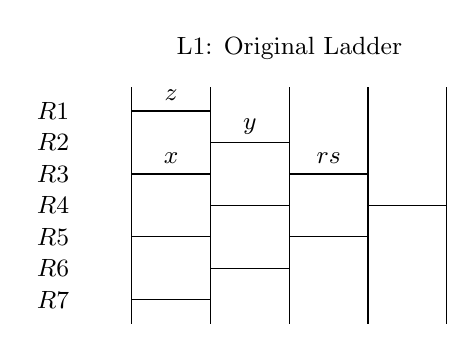
\begin{tikzpicture}
			\node at(2, 3.5){\small{L1: Original Ladder}};
			\draw(0, 0) to (0, 3);
					\node at(.5, 2.9){\small{$z$}};
				\draw(0, 2.7) to (1,2.7);
					\node at(.5, 2.1){\small{$x$}};

				\draw(0,1.9) to (1,1.9);
				\draw(0,1.1) to (1,1.1);
				\draw(0,0.3) to (1,0.3);
			\draw(1, 0) to (1, 3);
				\node at(1.5,2.5){\small{$y$}};
				\draw(1,2.3) to (2,2.3);
				\draw(1,1.5) to (2,1.5);
				\draw(1,0.7) to (2,0.7);
			\draw(2, 0) to (2, 3);
				\node at(2.5, 2.1){\small{$rs$}};
				\draw(2,1.9) to (3,1.9);
				\draw(2,1.1) to (3,1.1);
			\draw(3, 0) to (3, 3);
				\draw(3,1.5) to (4,1.5);
			\draw(4, 0) to (4, 3);

			\node at(-1, 2.7){\small{$R1$}};
			\node at(-1, 2.3){\small{$R2$}};
			\node at(-1, 1.9){\small{$R3$}};
			\node at(-1, 1.5){\small{$R4$}};
			\node at(-1, 1.1){\small{$R5$}};
			\node at(-1, .7){\small{$R6$}};
			\node at(-1, .3){\small{$R7$}};

			
		\end{tikzpicture}
	\end{minipage}
	\begin{minipage}{.4\textwidth}
		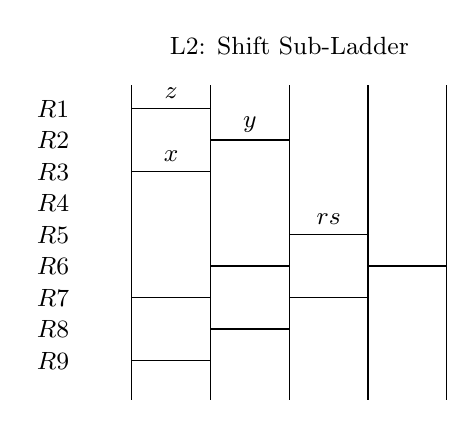
\begin{tikzpicture}
			\node at(2, 3.5){\small{L2: Shift Sub-Ladder}};

			\draw(0, -1) to (0, 3);
					\node at(.5, 2.9){\small{$z$}};
				\draw(0, 2.7) to (1,2.7);
					\node at(.5, 2.1){\small{$x$}};

				\draw(0,1.9) to (1,1.9);
				\draw(0,.3) to (1,.3);
				\draw(0,-0.5) to (1,-0.5);
			\draw(1, -1) to (1, 3);
				\node at(1.5,2.5){\small{$y$}};
				\draw(1,2.3) to (2,2.3);
				\draw(1,0.7) to (2,0.7);
				\draw(1,-0.1) to (2,-0.1);
			\draw(2, -1) to (2, 3);
				\node at(2.5, 1.3){\small{$rs$}};
				\draw(2,1.1) to (3,1.1);
				\draw(2,.3) to (3,.3);
			\draw(3, -1) to (3, 3);
				\draw(3,.7) to (4,.7);
			\draw(4, -1) to (4, 3);

			\node at(-1, 2.7){\small{$R1$}};
			\node at(-1, 2.3){\small{$R2$}};
			\node at(-1, 1.9){\small{$R3$}};
			\node at(-1, 1.5){\small{$R4$}};
			\node at(-1, 1.1){\small{$R5$}};
			\node at(-1, .7){\small{$R6$}};
			\node at(-1, .3){\small{$R7$}};
			\node at(-1, -.1){\small{$R8$}};
			\node at(-1, -.5){\small{$R9$}};


			
		\end{tikzpicture}
	\end{minipage}
		\begin{minipage}{.4\textwidth}
		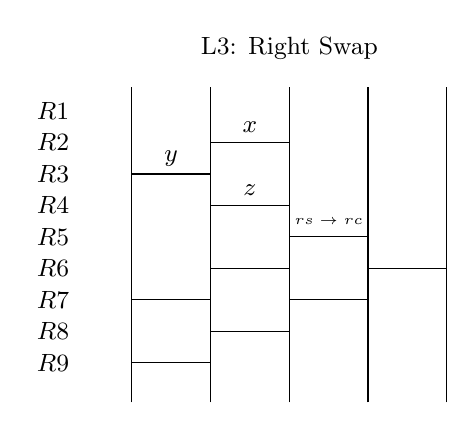
\begin{tikzpicture}
			\node at(2, 3.5){\small{L3: Right Swap}};

			\draw(0, -1) to (0, 3);
					\node at(1.5, 1.7){\small{$z$}};
				
					\node at(.5, 2.1){\small{$y$}};

				\draw(0,1.9) to (1,1.9);
				\draw(0,.3) to (1,.3);
				\draw(0,-0.5) to (1,-0.5);
			\draw(1, -1) to (1, 3);
				\node at(1.5,2.5){\small{$x$}};
				\draw(1,2.3) to (2,2.3);
				\draw(1, 1.5) to (2,1.5);
				\draw(1,0.7) to (2,0.7);
				\draw(1,-0.1) to (2,-0.1);
			\draw(2, -1) to (2, 3);
				\node at(2.5, 1.3){\tiny{$rs \rightarrow rc$}};
				\draw(2,1.1) to (3,1.1);
				\draw(2,.3) to (3,.3);
			\draw(3, -1) to (3, 3);
				\draw(3,.7) to (4,.7);
			\draw(4, -1) to (4, 3);

			\node at(-1, 2.7){\small{$R1$}};
			\node at(-1, 2.3){\small{$R2$}};
			\node at(-1, 1.9){\small{$R3$}};
			\node at(-1, 1.5){\small{$R4$}};
			\node at(-1, 1.1){\small{$R5$}};
			\node at(-1, .7){\small{$R6$}};
			\node at(-1, .3){\small{$R7$}};
			\node at(-1, -.1){\small{$R8$}};
			\node at(-1, -.5){\small{$R9$}};


			
		\end{tikzpicture}
	\end{minipage}
	\caption{$x,y,z$ to be right swapped. $rs$ is the right sibling; the root bar of the right sub-ladder.
	Going right to left, top to bottom. L1=original ladder, L2=shifting the right sub-ladder down two rows. L3 = right swap on $x,y,z$}
	\label{Fig:SwapAndShift}
\end{figure}

When a right swap operation is about to occur, bar $z$ will be moved from its current row and column to its current row + $3$ 
and its current column $+1$. Once the right swap opeartion is performed, 
the right sibling/$rs$ of $x$ becomes the right child/$rc$ of $z$.
The left swap operation is simply the inverse function of the right swap operation. 
Therefore, one can derive the left swap operation and the shift required for left swapping by deriving them 
from the right swap operation and the shift required for the right swap operation.

\begin{lemma}
	Shifting the entire sub-tree beginning at $rs$ down 
two rows ensures that $rs$ becomes $rc(z)$ and the ladder maintains its structure.
\end{lemma}
\begin{proof}
	Assume $ladder$ is a $1$ indexed two dimensional array. Going down the ladder is moving in the positive 
	direction and going up the ladder is moving in a negative direction. 
	Let $k$ be the current row of $z$. Let $k'=k+3$ be the target row of $z$. Let $m$ be the row of $rs$.
	We know that $m$ also equals the row of $x$ seeing as $rs$ is on the same row as $x$ prior to the 
	right swap operation. We know that $k$ = $m-2$ seeing as $z$ is two rows above $x$. Thus, 
	$k'=k+3=(m-2)+3=(m+1)$. Thus, the target row of $z=m+1$. Let $o$ be the current column of $z$.
	Let $o+1$ be the target column of $z$. We know that $o$ is 
	also the column of $x$ seeing as $z$ and $x$ are in the same column. 
	Thus, we know that the column of $rs$ is $o+2$ seeing as $rs$ is the right sibling  
	of $x$. Therefore the target destination of $z$ is $ladder[k'=m+1][o+1]$. 
	$rs$ is in the column $o+2$ and is at $row=m$ prior to the right swap opeartion. 
	We know that $rs \rightarrow rc(z)$ after the right swap operation, therefore $rs$ 
	must appear in the ladder at row $k'+1=m+1+1$ and the column of $o'+1$; please refer to theorem \ref{Theorem:One}
	for the definition of the right child. Since the column of $rs=o'+1$, then the column does not have to be changed.
	Since the current row of $rs$ is $m$, then the right sub-ladder needs to be shfited down by $+2$ to ensure 
	that $rs \rightarrow rc(z)$ after the right swap operation is performed. Since $rs$ also has right and left children, 
	each of them need to be shifted down two rows to ensure the ladder mainatins its structure whence the right swap 
	operation is performed. QED. 

\end{proof}

